\chapter{Launch and manage instances}\label{cha:launch-manage-inst}

Instances are virtual machines that run inside the cloud. You can launch
an \gls{instance} from the following sources:

\begin{itemize}
\item Images uploaded to the Image service.  Note that, because images
    are read-only, any changes made while the instance is running will
    be lost after shutdown, unless you choose to ``Create New
    Volume''.  If you create a new volume, the VM's state will persist
    after shutdown.
  \item Image that you have copied to a persistent volume. The instance
  launches from the volume, which is provided by the
  \textbf{cinder-volume} API through iSCSI.
\item Instance snapshot that you took.
\end{itemize}

\subsection*{Launch an instance}\label{launch-an-instance}

\begin{enumerate}
\def\labelenumi{\arabic{enumi}.}
\item Open the Compute tab and click Instances category.

  The dashboard shows the instances with its name, its private and
  floating IP addresses, size, status, task, power state, and so on.
\item Click Launch Instance.
\item In the Launch Instance dialog box, specify the following values:

  \begin{center}
    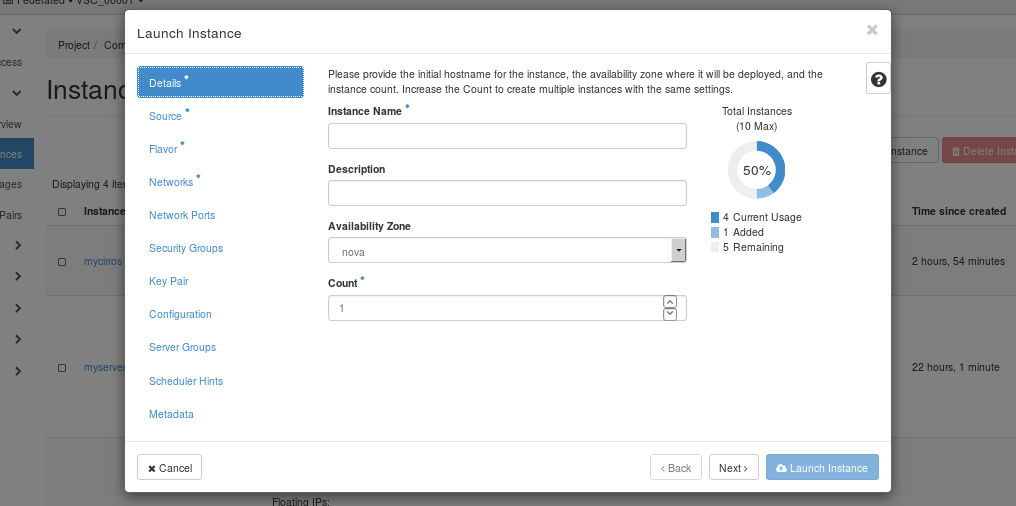
\includegraphics[scale=0.5]{img/tab-compute-instances-launch.png}
  \end{center}
  
  \begin{description}
  \item[Details] tab
    \begin{description}
    \item[Instance Name] Assign a name to the virtual machine.

      \strong{Note:} The name you assign here becomes the initial host
      name of the server. If the name is longer than 63 characters,
      the Compute service truncates it automatically to ensure dnsmasq
      works correctly.

      After the server is built, if you change the server name in the
      API or change the host name directly, the names are not updated
      in the dashboard.

      Server names are not guaranteed to be unique when created so you
      could have two instances with the same host name.

    \item[Description] You can assign a brief description of the
      virtual machine.
    \item[Availability Zone] By default, this value is set to the
      availability zone given by the cloud provider (for example,
      \strong{us-west} or \strong{apac-south}).  For some cases, it
      could be \strong{nova}.
    \item[Count] To launch multiple instances, enter a value greater
      than \strong{1}. The default is \strong{1}.
    \end{description}

    \begin{center}
      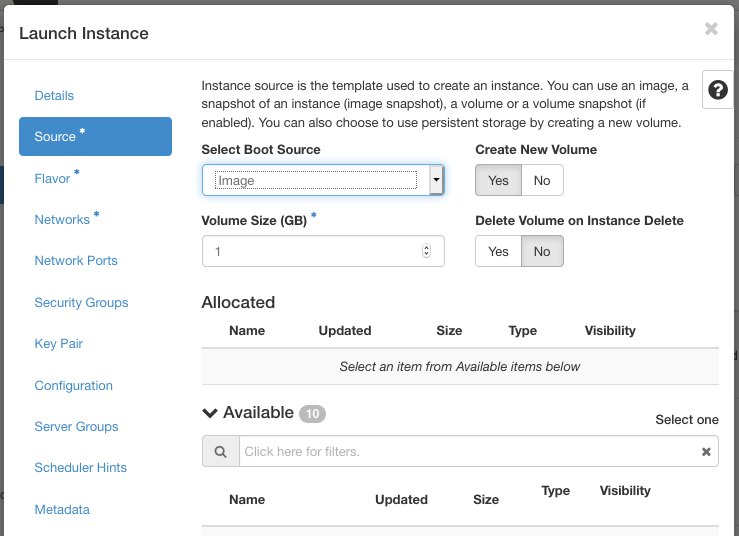
\includegraphics[width=0.7\textwidth]{img/launch_instance_source}
    \end{center}
  \item[Source] tab
  \begin{description}
  \item[Select Boot Source] Your options are:
    \begin{description}
    \item[Image]
    \item[Image snapshot]
    \item[Volume]
    \item[Volume snapshot]
    \end{description}
    Depending on the type of boot source, the list of available items
    changes.

  \item[Create New Volume] If you enable this option when launching
    from an image or instance snapshot, the image or snapshot will be
    copied to a volume.  This way, the state of your instance persists
    after shutdown and reboot.
  \end{description}

\item[Flavor] tab. Specify the size of the instance to launch.

  \strong{Note:} The flavor is selected based on the size of the image
  selected for launching an instance. For example, while creating an
  image, if you have entered the value in the Minimum RAM (MB) field
  as 2048, then on selecting the image, the default flavor is
  \textbf{m1.small}.

\item[Networks] tab. Add one or more networks to the instance.

\item[Network Ports] tab. Activate the ports that you want to assign to
  the instance.
\item[Security Groups] tab. Activate the security groups that you want
  to assign to the instance.

  Security groups are a kind of cloud firewall that define which
  incoming network traffic is forwarded to instances.

  If you have not created any security groups, you can assign only the
  default security group to the instance.

\item[Key Pair] tab. Specify a key pair.

  If the image uses a static root password or a static key set
  (neither is recommended), you do not need to provide a key pair to
  launch the instance.
\item[Configuration] tab. Specify a customization script that runs
  after your instance launches.

\item[Server Groups] tab.

\item[Scheduler Hints] tab.

\item[Metadata] tab. Add Metadata items to your instance.
\end{description}

\def\labelenumi{\arabic{enumi}.}
\item Click Launch Instance.
\end{enumerate}

The instance starts on a compute node in the cloud.

\strong{Note:} If you did not provide a key pair, security groups, or
rules, users can access the instance only from inside the cloud
through VNC. Even pinging the instance is not possible without an ICMP
rule configured.

You can also launch an instance from the Images or Volumes category when
you launch an instance from an image or a volume respectively.

When you launch an instance from an image, OpenStack creates a local
copy of the image on the compute node where the instance starts.

For details on creating images, see
\href{https://docs.openstack.org/image-guide/create-images-manually.html}{\emph{Creating
images manually}} in the \emph{OpenStack Virtual Machine Image Guide}.

\strong{Note:} When running QEMU without support for the hardware
virtualization, set \textbf{cpu\_mode="none"} alongside
\textbf{virt\_type=qemu} in \textbf{/etc/nova/nova-compute.conf} to
solve the following error:

libvirtError: unsupported configuration: CPU mode 'host-model'

for ``x86\_64`` qemu domain on ``x86\_64`` host is not supported by
hypervisor

\strong{Connect to your instance by using SSH}\label{connect-to-your-instance-by-using-ssh}

To use SSH to connect to your instance, use the downloaded keypair file.

\strong{Note:} The user name is \textbf{ubuntu} for the Ubuntu cloud
images on TryStack.

\begin{enumerate}
\def\labelenumi{\arabic{enumi}.}
\item Copy the IP address for your instance.
\item Use the \textbf{ssh} command to make a secure connection to the
  instance. For example:
\item \$ ssh -i MyKey.pem ubuntu@10.0.0.2
\item At the prompt, type \textbf{yes}.
\end{enumerate}

It is also possible to SSH into an instance without an SSH keypair, if
the administrator has enabled root password injection. For more
information about root password injection, see
\href{https://docs.openstack.org/nova/\osversion/admin/admin-password-injection.html}{\emph{Injecting the administrator password}} in the \emph{OpenStack Administrator
Guide}.

\strong{Track usage for instances}\label{track-usage-for-instances}

You can track usage for instances for each project. You can track costs
per month by showing meters like number of vCPUs, disks, RAM, and uptime
for all your instances.

\begin{enumerate}
\def\labelenumi{\arabic{enumi}.}
\item Open the Compute tab and click Overview category.
\item To query the instance usage for a month, select a month and click
  Submit.
\item To download a summary, click Download CSV Summary.
\end{enumerate}

\strong{Create an instance snapshot}\label{create-an-instance-snapshot}

\begin{enumerate}
\def\labelenumi{\arabic{enumi}.}
\item Open the Compute tab and click the Instances
  category.
\item Select the instance from which to create a snapshot.
\item In the actions column, click Create Snapshot.
\item In the Create Snapshot dialog box, enter a name for the snapshot, and
  click Create Snapshot.
\end{enumerate}

The Images category shows the instance snapshot.

To launch an instance from the snapshot, select the snapshot and click
Launch. Proceed with launching an instance.

\strong{Manage an instance}\label{manage-an-instance}

\begin{enumerate}
\def\labelenumi{\arabic{enumi}.}
\item Open the Compute tab and click Instances category.
\item Select an instance.
\item In the menu list in the actions column, select the state.
\end{enumerate}

You can resize or rebuild an instance. You can also choose to view the
instance console log, edit instance or the security groups. Depending on
the current state of the instance, you can pause, resume, suspend, soft
or hard reboot, or terminate it.

%%% Local Variables:
%%% mode: latex
%%% TeX-master: "intro-OpenStack"
%%% End:
